\documentclass{article}
\documentclass{article}
\usepackage[utf8]{inputenc}
\usepackage[T1]{fontenc}
\usepackage[french]{babel}
\usepackage[autolanguage]{numprint} % for the \nombre command
\usepackage{algorithm}
\usepackage{algorithmic}
\usepackage{amsmath}
\usepackage[margin=2cm]{geometry}
\usepackage{amsfonts}
\usepackage{amssymb}
\usepackage{hyperref}
\usepackage{graphicx}
\usepackage[euler]{textgreek}

\usepackage[style=ieee]{biblatex}
\addbibresource{LLP.bib}

%\newgeometry{top=2.5cm, left=2.5cm, right=2.5cm, bottom=2.5cm}

\hypersetup{
    colorlinks=true,
    linkcolor=blue,
    breaklinks=true,
    urlcolor= blue,
    citecolor = black,
}

\title{Solveur et générateur de sudoku}

\author{
  MOUSSA MOHAMED Abdoulkader
}
\date{Janvier 2023}

\begin{document}

\maketitle

\section{Introduction}
Ce rapport rentre dans le cadre de l'UE \textbf{Low-Level Programming} du semestre 1 qui a pour
objectif de nous apporter les connaissances et compétences de base nécessaires pour programmer en langage C. \vspace{0.3cm}

Nous avons, dans le cadre de cette UE, eté amené à programmer un solveur et un générateur  du fameux jeu \textbf{sudoku}. Le solveur sudoku permet de résoudre des grilles de différentes tailles (4, 9, 16, 25, 36, 49, 64) en donnant une ou toutes les solutions possibles. Le générateur, quant à lui, permet de créer des grilles de sudoku de différentes tailles. Il peut également créer des grilles qui ont une unique solution.
\vspace{0.3cm}

Dans un premier temps, nous verrons les stratégies appliquées dans le solveur sudoku , ce qui lui permet  d'avoir une meilleure performance.
Dans un second temps, nous verrons comment notre générateur génère des grilles(unique ou pas) et cela en temps raisonnable. 


\section{Solveur sudoku}

Dans cette partie, nous verrons les stratégies appliquées dans le solveur sudoku après le \textit{homework-5} et qui lui permettent d'avoir une meilleure performance:
\vspace{0.2cm}
\begin{enumerate}
    \item[$\ast$] \textbf{Réduction de la complexité des heuristique \textit{cross-hatching} et \textit{lone-number}: } \vspace{0.12cm} \newline
    Au \textit{homework-5}, les heuristique  \textit{cross-hatching} et \textit{lone-number} avaient une complexité de O(n²). Or, diminuer cette complexité est largement faisable. Nous avons donc réduit cette complexité et elle est desormais en O(n).\vspace{0.2cm}
    \item[$\ast$] \textbf{Reduction de la complexité de la fonction  \textit{grid\_choice()}: } \vspace{0.12cm} \newline
    La fonction \textit{grid\_choice()} retourne une couleur se trouvant dans le plus petit ensemble de couleur de toute la grille. La complexité temporelle de cette fonction a eté reduite passant de O(c * n²) à O(n²). (c variant de 1 à n). \vspace{0.12cm}
    \item[$\ast$] \textbf{Ajout d'une nouvelle hereustique \textit{locked-candidate}} \vspace{0.12cm} \newline
    Il existe plusieurs techniques avancées de sudoku(heuristique)  qui peuvent être utilisés dans les grilles complexes pour éliminer des candidats et permettre ainsi une résolution plus rapide.\vspace{0.2cm}

    Nous avons implémenté l'heuristique \textit{locked-candidate} de type \textit{pointing} . 
    
    La régle est la suivante \cite{locked_candidates_rules}:
    \textit{Si un candidat se trouve au moins deux fois sur une même ligne ou colonne uniquement, et à l’intérieur d’un même bloc, alors il peut être éliminé sur toute cette ligne ou colonne à l’extérieur du bloc.}  
    
    \vspace{0.12cm}.
    \begin{figure}[H]
    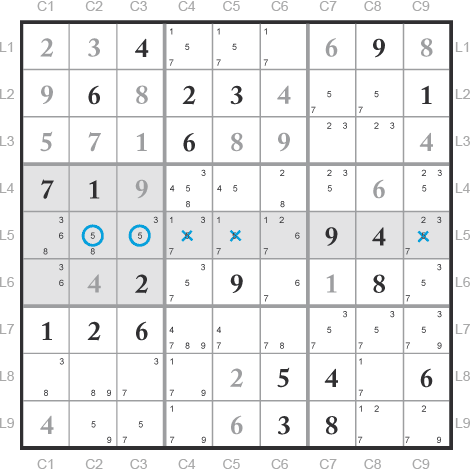
\includegraphics[width=9cm,left]{locked-candidate-row.png}
    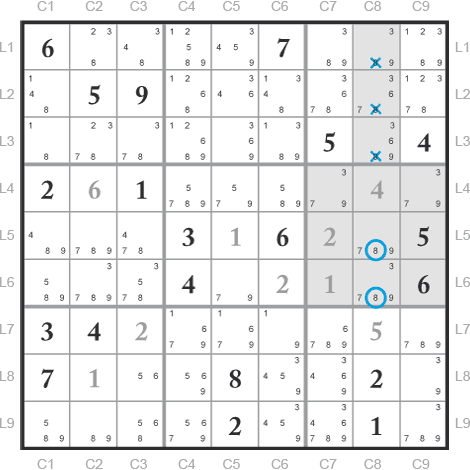
\includegraphics[width=9cm,right]{reduction3.png}
    \caption{\textit{locked-candidate-pointing} sur une ligne et colonne\cite{locked_candidates_rules}.}
\end{figure}

Cette heuristique n'a pas beaucoup d'effet sur les grilles de niveau facile ou de petite taille. Mais a beaucoup d'effet sur les grilles de niveau difficile ou de grande taille. \vspace{0.2cm}

Nous avons testé cela. Sans l'heuristique \textit{locked-candidate}, notre solveur met plus de 5 minutes à résoudre la grille 64x64-11.sku
 de niveau 4. Et ne met que 4 secondes avec cette dernière.\vspace{0.5cm}

\item[$\ast$] \textbf{Utilisés toutes les heuristiques en même temps peu être très couteux en temps : } \vspace{0.15cm}

Nous avons maintenant implémenté plusieurs heuristiques. En les utilisant toutes en même temps, nous avons une complexité temporelle trés importante. Or, notre principal objectif est d'avoir une complexité temporelle la plus minimale possible. On doit donc se servir stratégiquement de nos heuristiques. La figure 2 ci-dessous illustre cela. 

\begin{figure}[H]
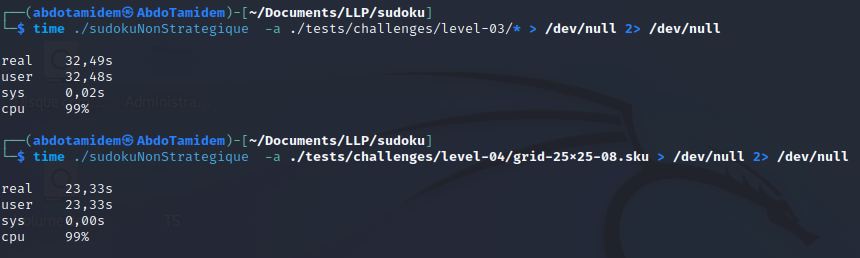
\includegraphics[width=9cm,left]{sansStrategie.png}
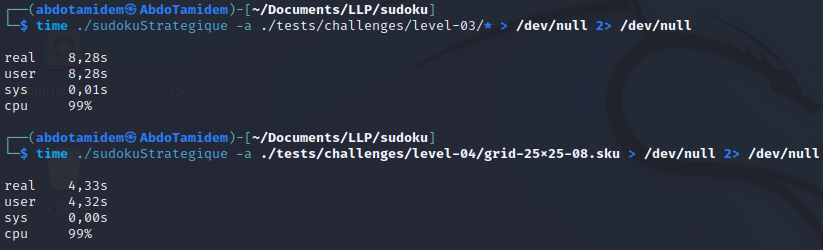
\includegraphics[width=9cm,right]{strategique.png}
    \caption{heuristique utilisés non strategiquement vs strategiquement}
\end{figure}

Voici les choix qui ont eté fait pour se servir stratégiquement de nos heuristiques:\vspace{0.2cm}

\begin{itemize}
    \item \textbf{Ne pas utiliser l'heuristique \textit{hidden-subset} :}
    
    Nous avons constaté qu'avec ou sans l'heuristique \textbf{hidden-subset}, notre solveur sudoku prend approximativement le même temps pour résoudre une grille. Comme cela ne nous fait pas gagner du temps, nous avons donc decider de ne pas l'utiliser.\vspace{0.2cm}

    \item \textbf{Appliquer l'heuristique  \textit{naked-subset} uniquement si la grille a changé après application des heuristique \textit{cross-hatching} et \textit{lone-number} }\vspace{0.4cm}

    \item \textbf{Moins utiliser l'heuristique  \textit{locked-candidate} :}

    Nous avons remarqué que restreindre l'utilisation de l'heuristique  \textit{locked-candidate} fait gagner du temps à notre solveur.
    C'est-à-dire l'appliquer sur la grille uniquement si la grille n'a pas changé après application des autres heuristiques.
    
    
\end{itemize}

\end{itemize}


\section{Générateur sudoku}

\subsection{Le solveur sudoku légèrement modifié }

Pour pouvoir génèrer une grille, nous avons besoin d'un solveur sudoku qui:
\vspace{0.1cm}
\begin{itemize}
    \item nous permet de savoir si une grille a \textbf{une} ou \textbf{plus d'une} solution.\vspace{0.1cm}
    \item retourne une des solutions trouvées.
\end{itemize}
\vspace{0.2cm}
Or, pour une grille donnée, notre solveur sudoku :
\vspace{0.1cm}
\begin{itemize}
    \item nous permet de savoir le nombre de solutions exactes.\vspace{0.1cm}
    \item affiche \textbf{une} ou \textbf{toutes} les solutions.
\end{itemize}
\vspace{0.2cm}

Alors, pour pouvoir génèrer une grille en temps raisonnable, nous avons faits une légére amélioration sur une copie du solveur:
\vspace{0.2cm}
\begin{itemize}
    \item Ajout d'une structure de type énumération \textbf{generator\_t} qui contient comme valeur \textit{mode\_unique} et  \textit{mode\_not\_unique}. Ceci nous permet de savoir quel type de grille nous devons génèrer.\vspace{0.15cm}
    \item Si la grille à génèrer est en \textit{mode\_not\_unique}, c'est-à-dire qu'elle ne doit pas avoir obligatoirement une unique solution, alors dès qu'une solution est trouvée, notre solveur peut s'arrêter et retourner la solution trouvé.\vspace{0.15cm}
    \item Si la grille à génèrer est en \textit{mode\_unique}, c'est-à-dire qu'elle doit avoir une unique solution, alors au bout de deux solutions trouver, notre  solveur peut s'arrêter. Ceci car ce qui nous interesse vraiment c'est de savoir s'il ya \textbf{une} ou \textbf{plus d'une} solution.\vspace{0.15cm}
    \item Le solveur ne doit absolument rien afficher..\vspace{0.15cm}
    \item Ne pas appliquer l'heuristque \textit{locked\_candidates} sur la grille. Car cela ralenti énormement notre génèrateur.
\end{itemize}

\subsection{ Fonctionnement du génèrateur }

  \subsubsection{ Génèrateur en \textit{mode\_not\_unique} }

Pour génèrer une grille en \textit{mode\_not\_unique}, notre générateur suit les étapes suivantes:

\begin{enumerate}
    \item Créer une grille dont toutes les cases sont masquées(contiennent toutes les valeurs possibles). Puis on fixe une valeur dans une case aléatoirement. Ceci nous permet d'avoir une nouvelle grille à chaque fois. \vspace{0.15cm}
    \item On utilise notre nouveau solveur pour trouver une solution à cette grille. Notre nouveau solveur va s'arreter à la premiere solution trouvée .\vspace{0.15cm}
    \item On masque $40\%$ des cases.  \vspace{0.15cm}
\end{enumerate}

\textbf{Temps d'execution en fonction de la taille de la grille}
\vspace{0.2cm}

\begin{itemize}
    \item[$\ast$] Taille 4: 0.00s \vspace{0.12cm}
    \item[$\ast$] Taille 9: 0.01s \vspace{0.12cm}
    \item[$\ast$] Taille 16: 0.01s \vspace{0.12cm}
    \item[$\ast$] Taille 25: 0.03s \vspace{0.12cm}
    \item[$\ast$] Taille 36: 0.18s \vspace{0.12cm}
    \item[$\ast$] Taille 49: 0.34s \vspace{0.12cm}
    \item[$\ast$] Taille 64: 1.10s \vspace{0.12cm}
\end{itemize}
 \vspace{1cm}
 
\textbf{Analyse de la complexité temporelle}\vspace{0.13cm}

 
Soit n la taille de la grille à génèrer.
\vspace{0.18cm}

\textbf{Etape 1:} O(n²) car nous devons parcourir toutes les cases de la grilles pour pouvoir les masquer. Fixer une valeur à une case: O(1).\vspace{0.15cm}

\textbf{Etape 2:} Depend vraiment de n et du niveau de difficulté de la grille à résoudre.\vspace{0.15cm}

\textbf{Etape 3:} O(n).\vspace{0.15cm}
  
\subsubsection{ Générateur en \textit{mode\_unique} }

Pour génèrer une grille en \textit{mode\_unique}, notre générateur suit les étapes suivantes:
\vspace{0.2cm}
\begin{enumerate}
    \item Créer une grille dont toutes les cases sont masquées(contiennent toutes les valeurs possibles). Puis on fixe une valeur dans une case aléatoirement. Ceci nous permet d'avoir une nouvelle grille à chaque fois. \vspace{0.15cm}
    \item On utilise notre nouveau solveur pour trouver une solution à cette grille. Notre nouveau solveur va s'arreter au bout de deux solutions trouvées. \vspace{0.15cm}
    \item On masque une case à la fois, aléatoirement. \vspace{0.15cm}
    \item A chaque fois qu'une case est masquée, nous lancons notre nouveau solveur sur la grille pour savoir combien de solutions nous avons. \vspace{0.15cm}
    \item Si la grille a une solution alors nous pouvons poursuivre le processus de l'étape 3. Sinon, nous remettons la valeur que nous avons retirée dans la grille. \vspace{0.15cm}
    \item Nous pouvons repeter le meme processus de l'etape 3 plusieurs fois jusqu'à masquer 40\% des cases. \vspace{0.15cm}
    
\end{enumerate}

Les deux premières étapes sont identiques quelques soit la grille à génèrer. \vspace{0.15cm}

\textbf{Temps d'execution en fonction de la taille de la grille}
\vspace{0.2cm}

\begin{itemize}
    \item[$\ast$] Taille 4: 0.00s \vspace{0.12cm}
    \item[$\ast$] Taille 9: 0.01s \vspace{0.12cm}
    \item[$\ast$] Taille 16: 0.01s \vspace{0.12cm}
    \item[$\ast$] Taille 25: 0.05s \vspace{0.12cm}
    \item[$\ast$] Taille 36: 0.31s \vspace{0.12cm}
    \item[$\ast$] Taille 49: 0.93s \vspace{0.12cm}
    \item[$\ast$] Taille 64: (prend un peu de temps) \vspace{0.12cm}
\end{itemize}
\vspace{0.2cm}

\textbf{Analyse de la complexité}\vspace{0.13cm}

 
Soit n la taille de la grille à génèrer.
\vspace{0.18cm}

\textbf{Etape 1 et 2:} Même complexité que les etapes 1 et 2 pour les grilles en mode\_not\_unique. \vspace{0.15cm}

\textbf{Etape 3:} O(1).\vspace{0.15cm}

\textbf{Etape 4:} Complexité du nouveau solveur sudoku   \vspace{0.15cm}

\textbf{Etape 5:} O(1).\vspace{0.15cm}

\textbf{Etape 6:} O($\frac{n}{2}$).\vspace{0.15cm}

\section{Conclusion}

Comme nous avions plusieurs heuristiques, il fallait faire des choix et les utiliser stratégiquement.
Nous avons donc vu les differentes strategies appliquées dans notre solveur sudoku et qui lui permettent ainsi d'avoir une bonne performance.  

Nous avons également vu comment notre programme arrivait à génèrer des grilles en temps raisonnable.

\selectlanguage{english}

\printbibliography

\end{document}

